\subsection{RAM access time}

To measure RAM access time, we followed the methodology used in section 6.2 of the LmBench paper \cite{lmbench}. We created arrays of increasing sizes and iterated through them 1 000 000 times sequentially and would wrap around if we reached the end of the array. Each such array is created at the beginning of an experiment and freed at the end. Thus, it has only one name, \texttt{array}. The contents of the arrays are filled as follows :

\begin{lstlisting}
for (int i = 0; i < size; i++)
  pA[i] = &pA[stride+i];
char* p = pA[0];
\end{lstlisting}

This way, the array can be traverse using the statement \texttt{p = *p;} according to the stride. The size of the arrays created varies from 32KB ($2^{15}$) to 256MB ($2^{28}$). For each array size, strides 16,64,256 and 1024 are profiled. 

In terms hardware performance, our system has two 32kB L1 caches , 2 256kB L2 caches and 1 3MB L3 cache. From our vendor \cite{vendor}, we known that our cache lines are 128 bytes. In terms of software overhead, we attempted to minimize the effect of loop overhead by using loop enrolling on the \texttt{p = *p;} statement.

The result of our experiment is shown on figure \ref{fig:b2blatency}. The resulting graph is similar to the one found in the LmBench paper. The transition from L1 cache to L2 cache and L3 cache to main memory are clearly visible and present where expected. The transition from L2 cache to L3 cache isn't noticeable, however. We also notice that when the stride size becomes greater than the cache line of the hardware, the main memory latency is greatly increased.

\begin{figure}
 \centering
  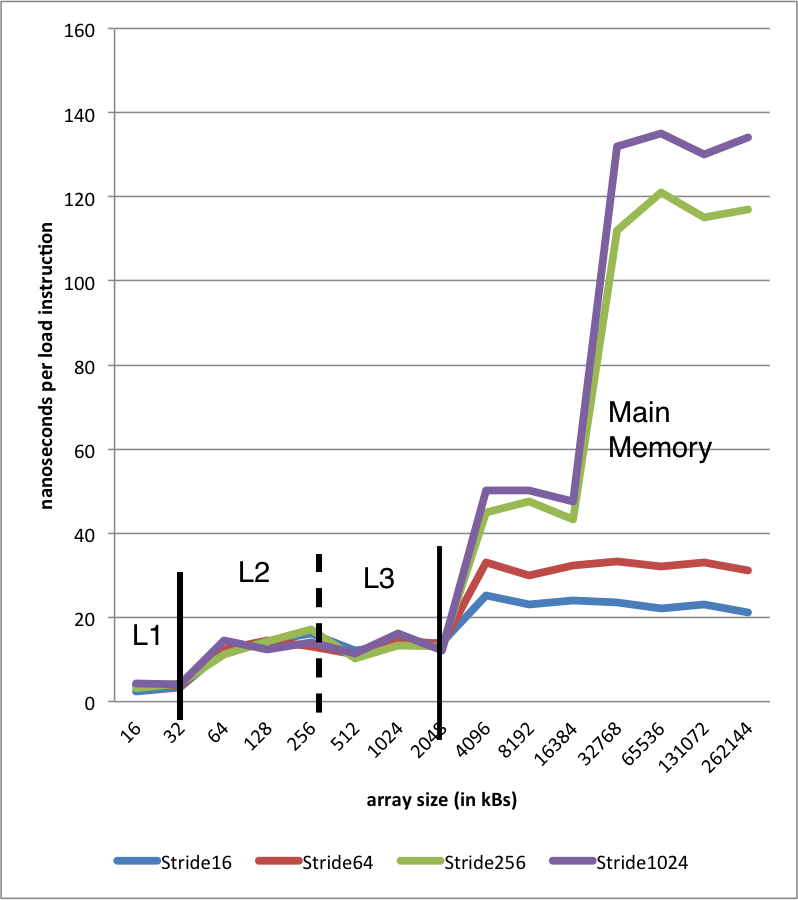
\includegraphics[width=0.5\textwidth]{image/backtobackload2.png}
  \caption{Back To Back Load Latency}
 \label{fig:b2blatency}
\end{figure}

\subsection{RAM bandwidth}

To measure RAM bandwidth, we followed the methodology suggested by the LmBench paper. However, we used the \texttt{mempcy} function since the \texttt{bcopy} function used in the paper has been deprecated since.

\subsubsection{RAM read bandwith}

For the read bandwidth, we created two arrays (of type \texttt{char}), called \texttt{bigArrayR} (162MB) and \texttt{smallArray} (3MB). \texttt{bigArray} is filled with random data before the beginning of the profiling (using \texttt{rand()}). When profiling starts, the contents of \texttt{bigArrayR} are sequentially read into \texttt{smallArray} in chunks of 3MB using \texttt{memcpy}  (in an enrolled loop).

The small array has been chosen to be exactly of the size of our L3 cache. After being repeatedly written into, it is expected that it will fill the contents of the cache, and all reads from \texttt{bigArrayR} are expected to originate from RAM. In terms of hardware performance, according to our vendor \cite{lenovo}, our RAM has a 10GB/s copy bandwidth. In terms of software overhead, according to the LmBench paper, pure read represents only about one half to one third of the \texttt{memcpy} work. Therefore, we can expect read bandwidth to run at twice the speed of a \texttt{memcpy} procedure call.

We obtained a read bandwidth by multiplying by 2.5 the time taken for reading the entire \texttt{bigArrayR} (averaged over 5 runs). This gives us a RAM read bandwidth of 13.62 GB/secs.

\subsubsection{RAM write bandwidth}

For the write bandwidth, we keep \texttt{smallArray} and create a new empty array \texttt{bigArrayW} (162MB), left empty this time. When profiling starts, contents from \texttt{smallArray} are sequentially written into \texttt{bigArrayW} in chunks of 3MB using \texttt{memcpy} in an enrolled loop.

After being repeatedly read from, it is expected that the contents of \texttt{smallArray} will fill the L3 cache, and all writes to \text{BigArrayW} will be written to RAM. Hardware performance and software overhead remain the same.

We obtained a read bandwidth by multiplying by 2.5 the time taken for write to the entire \texttt{bigArrayW} (averaged over 5 runs). This gives us a RAM write bandwidth of 8.90 GB/secs. This confirms the 10GB/s RAM copy bandwidth advertised by our vendor. Notice that read bandwidth is slightly higher than write bandwidth. One possible reason for this is given in the LmBench paper: in some processors, \emph{write transaction turns into a read followed by a write to maintain cache consistency}.

\subsection{Page Fault Service Time}

To profile page faults, we have used a mechanism proper to the Linux operating system called \textbf{Cgroups}. Cgroups are "tags" which can be specified when running process and which indicate to the operating system that only a restricted set of resources (indicated in the Cgroup description) should be allocated to the process. For example, we have restricted the amount of RAM used by the process for this experiment to 75MB.

In the experiment, we proceed to allocate an array (called \texttt{mallocs}) of 150 strings, each 1MB long. In order to ensure that the memory is actually allocated, we fill these 1MB strings with actual data. The memory allocation is done sequentially (the string for \texttt{mallocs[0]} is constructed before the string for \texttt{mallocs[1]} and so on...).

\begin{figure}
 \centering
  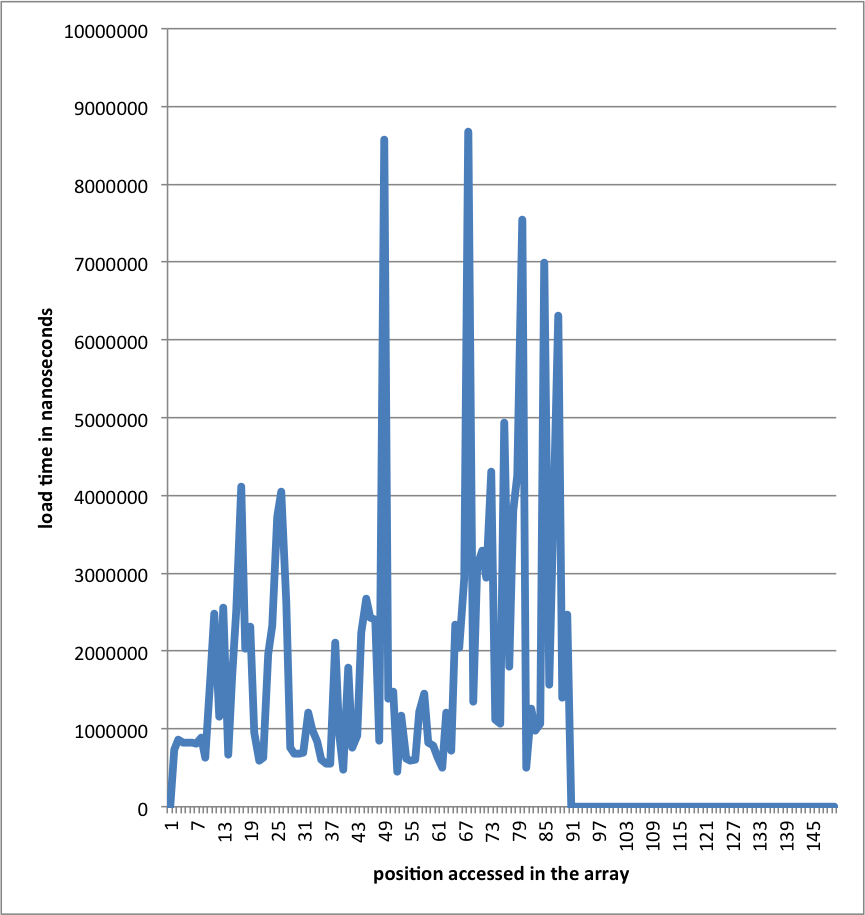
\includegraphics[width=0.5\textwidth]{image/pagefault.png}
  \caption{Page faults when accessing 150MB array}
 \label{fig:pagefault}
\end{figure}

Given the process can only 75MB of RAM, we can expect that at least half of the pages used by the \texttt{mallocs} array have been flushed to disk. Given data has been allocated sequentially, we can expect (according to the LRU rule), that these pages correspond to the first half of the array. The hardware performance of our SSD has been given by our vendor as a 750MB/sec read bandwidth. Software overhead is expected to be negligible in this experiment. However, in the context of a page fault, we can expect that after waiting for a while the OS might decide to do a context switch before coming back. Such context switch could occur while the process is waiting for a load instruction which is being profiled. As such, some fringe values in the experiment are to be expected as well.

These expectations are confirmed on figure ~\ref{fig:pagefault}. In this figure, we measure the time required to load each of the 1MB strings sequentially using \texttt{memcpy()} (we start by loading \texttt{mallocs[0]} and finish with \texttt{mallocs[149]}). We consider the 8-9 millisecond load times as the kind of fringe values we have to expect.
Given that the page size of our system is 4KB, 1MB corresponds to 256 pages. The median page load time for the first 90 MB is 1213/256 = 4.73  microseconds (which is consistent with the 750MB/sec bandwidth of our SSD). On the other hand, the average page load time for the last 60 MB is 0.8/256 = 0.00313  microseconds. This corresponds to a roughly 2000x increase when fetching pages from disk rather than main memory!

